\section{System Architecture}
\label{sa}
\todo{Figures}

\begin{figure}
    \centering
    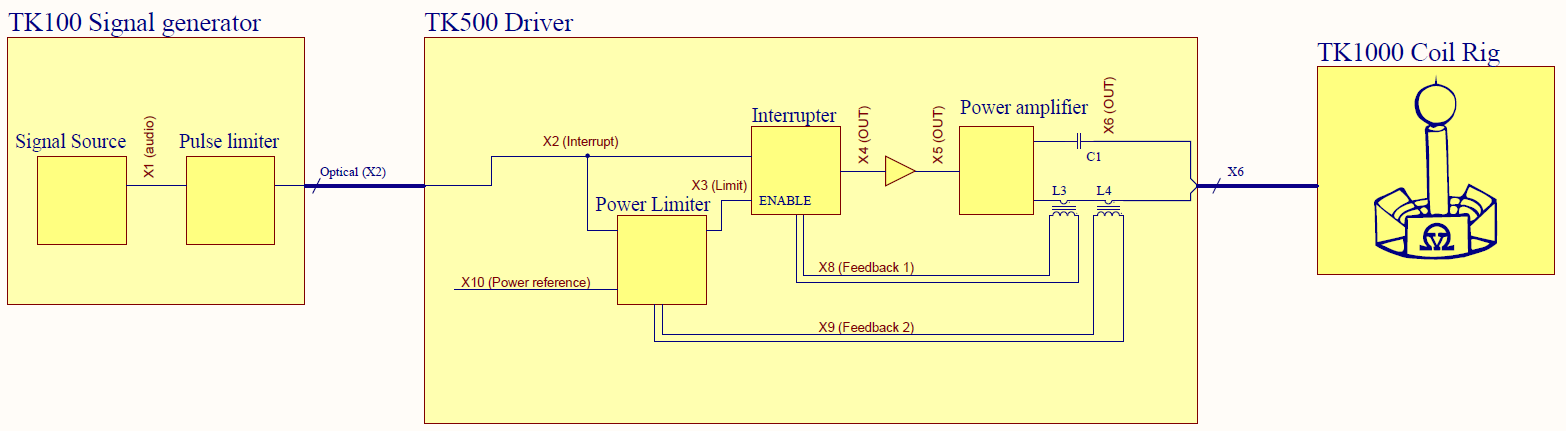
\includegraphics[width=\textwidth]{img/Blokkdiagram_detalj.PNG}
    \caption{Block diagram}
    \label{fig:blokksjema}
\end{figure}
To achieve the goal of high maintainability a back plane architecture was chosen. The choice of back plane is also defended as a way to eliminate wires and connectors between different pcbs, as wires can fall out during transport, and glue is not an alternative as it should be easy to change a module. The backplane provides a good electrical and mechanical connection as well as some additional features. \todo{Revise sentence, move someplace else?}

The signal source needs to be a long distance away from the coil rig due to safety reasons, and the power amplifier needs to be as close to the coil rig as possible to keep ohmic losses in the resonant circuit as low as possible. The Interrupter and power limiter has low voltage feedback signals X8 and X9 as inputs. Because of the nature of a tesla coil, there is a lot of electromagnetic interference (EMI) present such that low voltage signals needs to be sent through a channel that is robust against electromagnetical noise. Thus the system is partitioned such that the signal source and pulse shaper TK100 is placed together, and the rest of the system placed together in a shielded enclosure TK500. The signal from the pulse shaper X2 should then be sent through a robust channel. Optical plastic fibre is chosen described in \cref{optical}. X8 and X9 are then short and inside a shielded enclosure, and no other protection from EMI is required.

Inside TK500 we have both high power and low power signals. These should be separated such that the high power signals does not provide interference for the low power signals. And so that the electronics with low power signals can be designed with lower voltage and power requirements. This is solved by creating a signal back plane TK510 and a power back plane TK530, connected via an galvanic isolation TK520.

In addition some user interface is needed on the driver TK500 This is partitioned into a sub system called TK540.

%Bus on back plane, pros: can insert card anywhere cons: risk of inserting two of one card.

 
\subsection{Card inserted bus}
\label{section:ci}
When partitioning the system into several modules physically spread over multiple pcbs there is a risk of one module not being connected to the system, either because of issues with transportation, or by human error. To mitigate this risk, detection of wich cards is inserted into the back plane is implemented. This is done by a bus.
The bus consists of one wire named Card\_inserted, pulled high by a $10k\Omega$ resistor, \cref{fig:ki_bi} shows how each card slot interfaces to the card inserted bus, S1D shorted when a card is inserted and Card\_iserted is the bus. When no card is inserted into the slot the gate of the nmos is pulled high by R1 and the nmos goes into the triode region and pulls the bus low. When a card is inserted it pulls the gate low. And the nmos goes into cut-off. This circuit is replicated at each card slot.

\begin{figure}[h]
    \centering
    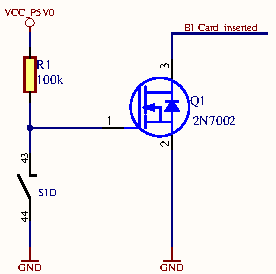
\includegraphics[width=8cm]{img/KI_BUS.pdf}
    \caption{Bus interface}
    \label{fig:ki_bi}
\end{figure}

\subsection{Optical channel}
\label{optical}

As mentioned in \cref{sa} a robust channel is needed for signal X2. For this plastic optical fibre is chosen. To further increase the robustness the signal (X2) should be modulated. To reduce complexity a simple modulation should be chosen. To remove the failure source of the optical cable missing (F3) and possibly some cases of defective optical cable (F2) the carrier wave (CW) should be chosen so that it is easily detectable in the receiving end.

\begin{figure}
    \centering
    \tikzstyle{int}=[draw, fill=yellow!20, minimum size=2em]
    \tikzstyle{init} = [pin edge={to-,thin,black}]
    \begin{tikzpicture}[node distance=2.5cm,auto,>=latex']
        \node [int, pin={[init]above:$CW$}] (a) {tx};
        \node (b) [left of=a,node distance=2cm, coordinate] {a};
        \node [int] (c) [right of=a] {rx};
        \node [int] (d) [left of=a] {TK100};
        \node [int] (e) [right of=c] {TK500};
        \node [coordinate] (end) [right of=c, node distance=2cm]{};
        \path[->] (d) edge node {$X2$} (a);
        \path[->] (a) edge node {$PWM$} (c);
        \draw[->] (c) edge node {$X2$} (e) ;
    \end{tikzpicture}
    \caption{Diagram of optical channel}
    \label{fig:my_label}
\end{figure}

\subsubsection{Carrier wave}
\label{carrier_wave}
The carrier wave CW for the optical channel should have a sufficiently high frequency $f=\frac{1}{T}$ to transfer the triggering signal X2, in addition to be easily detected in the receiving end. X2 contains two parts of information the positive flank determining when the tesla coil fires. and the duration of the positive pulse determining the power output (volume). The period $T$ should be shorter than the lowest desirable positive pulse on X2 $T_{X2min}$. \todo{Double check value from experiment} $f_{CW} > \frac{1}{T_{X2min}}$
The shortest desirable pulse on X2 is a length that allows turning the volume down without a noticeable step before shutoff.

\subsubsection{Modulation}
\label{modulation}
The triggering signal should be pulse width modulated PWM with a logical high having a duty cycle of 80\% and logical low having a duty cycle of 20\%.
\begin{figure}[h!]
    \centering
    \begin{tikztimingtable}
        CW & L 17{2C} G 1L \\
        $X2$ & 9L 8H 19L \\
        PWM & 1L 1H 3L 1H 3L 3H 1L 3H 1L 1H 3L 1H 3L 1L 1H 3L 1H 3L 1L 1H \\
    \end{tikztimingtable}
    \caption{Modulated signal timing diagram}
    \label{fig:cs_td}
\end{figure}{}

\subsection{Bus}
\label{bus}
\begin{figure}[h]
    \centering
    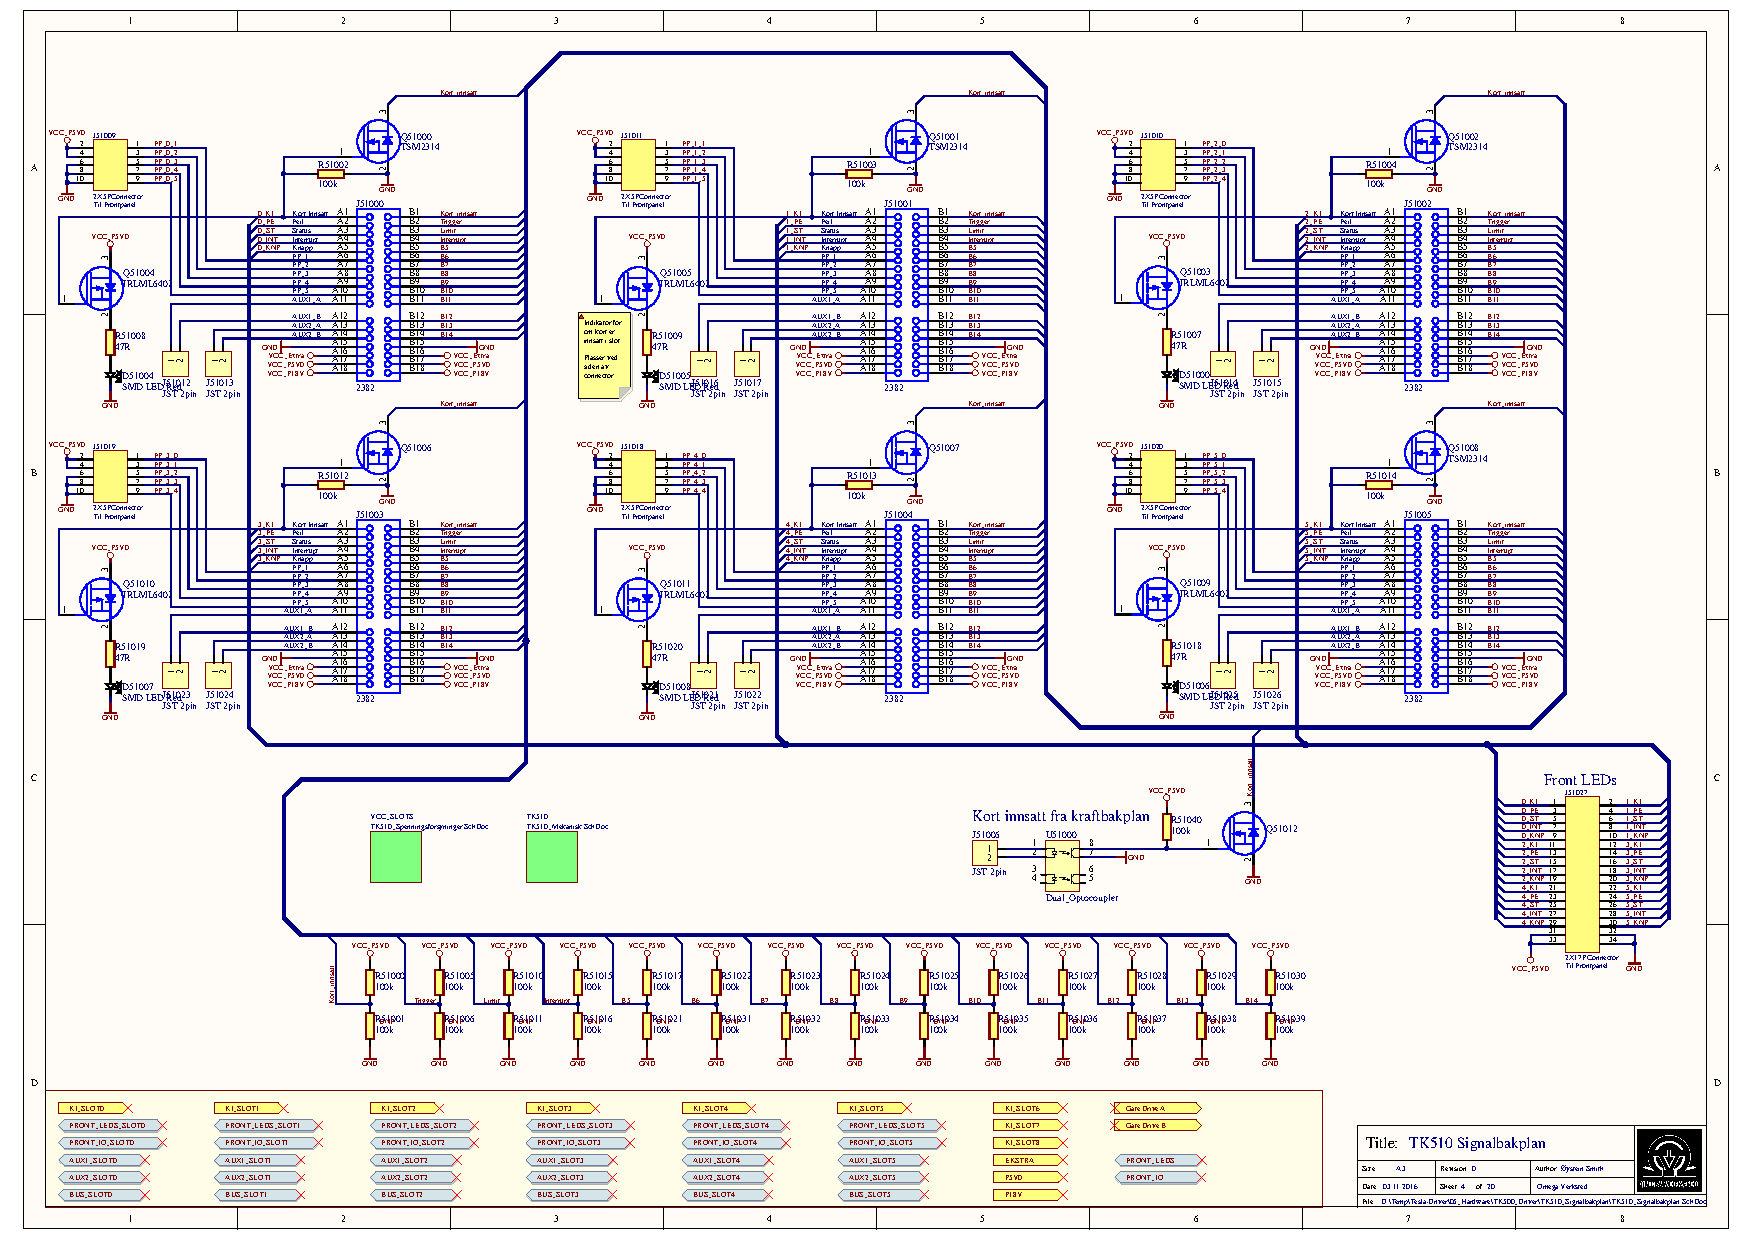
\includegraphics[trim={4.1cm 14.3cm 21.2cm 3.3cm},clip,width=\textwidth]{img/TK510_Signalbakplan.pdf}
    \caption{Signal module card slot connector (detail from schematic of TK510 Signalbakplan)}
    \label{fig:signalmodulslot}
\end{figure}
A set of signals should be available to all card slots on the signal back plane these signals are signals $B1$ to $B14$ in \cref{tab:bus}. The reason these signals should be present on all connectors is so that any module can be inserted in any slot of the back plane. In addition some unique signals should be present on each connector these are the other signals in \cref{tab:bus}. Signals n\_KI, n\_FE, n\_ST, and n\_INT are signals wich should drive leds on the front panel to indicate status of the module to the operator. The signal 0\_KNP should be connected to a button on the front panel for each card module slot on the signal back plane, for the operator to give simple feedback to the module.The signals FP\_1 to FP\_5 are signals to the front panel reserved for future use. The signals AUX1\_A \& AUX1\_B and AUX2\_A \& AUX2\_B are connectors used for the signals $X5$, $X8$, $X9$, $X10$ and the PWM signal from the optical channel, and added to all slots so that any module can be inserted into any slot, given that the aux connections are connected at the correct slot. The pinout of the connector is shown in \cref{fig:signalmodulslot}
\begin{table}[h!]
    \centering
    \begin{tabular}{|p{0.20\textwidth}|p{0.70\textwidth}|}
        \hline
        Signal name & Description \\ \hline
        B1 Card\_inserted & The card inserted bus described in \cref{section:ci} \\ \hline
        B2 Trigger & The triggering signal $X2$ \\ \hline
        B3 Limit & The output from the power limiter $X3$ \\ \hline
        B4 Interrupt & The output from the interrupter $X4$ \\ \hline
        B5 to B14 & Reserved for future use \\ \hline
        n\_KI & Card inserted (low when card is inserted floating otherwise as described in \cref{section:ci}) \\ \hline
        n\_FE & Active when fault detection of module detects a fault \\ \hline
        n\_ST & A status signal from the module \\ \hline
        n\_INT & Interrupt signal from the module, low when the module accepts the system firing, high otherwise. \\ \hline
        n\_KNP & Button input to the module from the front panel\\ \hline
        FP\_1 to FP\_5 & Signals to the front panel reserved for future use\\ \hline
        AUX1\_A & 'A' branch of, Auxillary input/output to the module terminated in a connector close to the card slot connector.\\ \hline
        AUX1\_B & 'B' - branch of AUX1\\ \hline
        AUX2\_A & Same as AUX1\\ \hline
        AUX2\_B & Same as AUX1 \\ \hline
    \end{tabular}
    \caption{Backplane signals.}
    'n' is the id of the connector slot
    \label{tab:bus}
\end{table}
